\documentclass[runningheads]{llncs}

\usepackage{url}
\usepackage{graphicx}
\usepackage{amsmath,amssymb}
\usepackage{booktabs}
\usepackage{multirow}
\usepackage{microtype}

\def\UrlFont{\rmfamily}
\def\UrlBreaks{\do\/\do\a\do\b\do\c\do\d\do\e\do\f\do\g\do\h\do\i\do\j\do\k\do\l\do\m\do\n\do\o\do\p\do\q\do\r\do\s\do\t\do\u\do\v\do\w\do\x\do\y\do\z\do\A\do\B\do\C\do\D\do\E\do\F\do\G\do\H\do\I\do\J\do\K\do\L\do\M\do\N\do\O\do\P\do\Q\do\R\do\S\do\T\do\U\do\V\do\W\do\X\do\Y\do\Z\do0\do1\do2\do3\do4\do5\do6\do7\do8\do9\do\-\do\_}

\begin{document}

\title{Federated SHAP: Privacy-Preserving, Per-Node Explainability and Sensitivity Analysis for Pediatric Sepsis Prediction}

\titlerunning{Federated SHAP for Pediatric Sepsis Prediction}

% Camera-Ready Author and Institute Information (Springer LNNS)
\author{Tanish Porwal\inst{1}\thanks{These authors contributed equally to this work.} \and
Uzair Teli\inst{1}\fnmsep\thanks{These authors contributed equally to this work.} \and
Praveen Modi\inst{1}}

\authorrunning{T. Porwal et al.}

\institute{Department of Engineering, SVKM's NMIMS Indore Campus, Indore, India\\
\email{\{tanishporwal2005,uzairteli7\}@gmail.com, praveen.modi@nmims.edu}}

\maketitle

\begin{abstract}
Federated learning enables multi-hospital pediatric sepsis prediction without centralizing patient records, but a federated model remains a black box to the clinicians who must act on it: federation solves privacy, not trust. We present a federated SHAP explainability pipeline that computes Shapley attributions \emph{locally} at each of five simulated ICU-type nodes on a shared global model, aggregates them using the same sample-size weighting FedAvg itself uses for model updates, and never transmits raw patient data or per-patient attributions off a node. On a Feature Tokenizer Transformer trained via FedAvg and FedProx across non-IID ICU nodes derived from the Pediatric Intensive Care (PIC) database with Phoenix Sepsis Criteria labelling, we find that \texttt{lactate\_max} is the unanimous top feature at all five nodes, and every node's local SHAP ranking correlates strongly with the federated aggregate (Spearman $\rho$ between 0.930 and 0.974 across all five nodes, including the smallest node, CICU, 5.7\% of training data, and the largest, General ICU, 49.4\%). FedAvg and FedProx further agree on 4 of their top 5 federated features ($\rho = 0.689$, $p = 5.4\times10^{-33}$). These results indicate that per-node federated explainability is both computationally practical and robust to severe non-IID node-size imbalance, at least along the algorithm-choice axis evaluated here.
\keywords{federated learning \and explainable AI \and SHAP \and pediatric sepsis \and Phoenix criteria \and privacy-preserving machine learning}
\end{abstract}

\section{Introduction}\label{sec:intro}

Pediatric sepsis progresses from suspected infection to multi-organ failure within hours, and delays in recognition of even one hour are associated with measurably higher mortality. An estimated 25 million pediatric sepsis cases occur annually worldwide, with mortality ranging from approximately 4\% in mild presentations to over 50\% in septic shock. To diagnose this condition, the Phoenix Sepsis Criteria established by Sanchez-Pinto et al. \cite{sanchezpinto2024phoenix} and Schlapbach et al. \cite{schlapbach2024phoenix} superseded prior SIRS-based definitions by Goldstein et al. \cite{goldstein2005sirs} by establishing explicit diagnostic thresholds across cardiovascular, coagulation, respiratory, and neurological systems, serving as the ground-truth labelling framework in this study.

Federated learning (FL) offers a compelling paradigm for collaborative training of sepsis risk estimators across distributed medical centers without moving confidential electronic health records off-site---a prerequisite enforced by stringent clinical data privacy mandates. The Federated Averaging (FedAvg) algorithm proposed by McMahan et al. \cite{mcmahan2017fedavg} and the FedProx framework developed by Li et al. \cite{li2020fedprox} serve as the primary decentralized optimization methods analyzed in this investigation. Nevertheless, privacy-preserving training guarantees confidentiality only during model synthesis; it fails to provide clinical transparency for the learned decision boundaries. A clinician at a small-volume Cardiac ICU node has no way to verify that a model trained mostly on a much larger General ICU node's patients is reasoning correctly about their own, potentially very different, patient population.

This is the specific gap this paper addresses. The SHAP framework introduced by Lundberg and Lee \cite{lundberg2017shap} is the standard framework for post-hoc model explanation in clinical machine learning, and is increasingly treated as a precondition for deploying high-risk medical AI, as surveyed by Athukorala and Ilmini \cite{athukorala2026explainable}. But SHAP explainability work in the sepsis literature has, to date, only ever been applied to centralized models trained on pooled data, such as recent work by Chanci et al. \cite{chanci2025machine}. No published study combines federated training with \emph{federated} explainability -- i.e., SHAP computed locally at each participating site and aggregated without any node's raw data or per-patient attributions ever leaving that site.

\subsubsection{Contributions.} This paper makes four main contributions:
\begin{enumerate}
\item A federated SHAP pipeline that computes GradientSHAP locally at each node and aggregates it with the same sample-size weighting FedAvg uses for model updates;
\item An empirical evaluation showing that per-node explanations agree strongly with the federated aggregate despite severe non-IID node-size imbalance (one node holds 49.4\% of all training data, another only 5.7\%);
\item A sensitivity analysis confirming this agreement is not an artifact of the choice of federated optimization algorithm; and
\item A fully specified privacy boundary detailing precisely what is and is not transmitted off a node at explanation time, not just at training time.
\end{enumerate}

\section{Literature Review}\label{sec:litreview}

\subsection{Pediatric Sepsis Prediction}
Machine learning applications in critical care sepsis diagnosis have expanded rapidly, with broad literature surveys indexing upward of 150 unique predictive models, such as comprehensive meta-analyses by Fleuren et al. \cite{fleuren2020ml} and Yang et al. \cite{yang2023sepsis}. The vast majority of published benchmarks concentrate on adult critical care repositories like MIMIC-III and MIMIC-IV, whereas investigations dedicated to pediatric demographics remain infrequent. Le et al. \cite{le2019pediatric} developed an early pediatric-focused severe sepsis predictor using institutional PICU records from UCSF, but operated without decentralized or privacy-preserving mechanics. Deng et al. \cite{deng2022evaluating} identified that subtle target leakage and fragile validation schemes remain pervasive shortcomings across critical care predictive modeling, issues our pipeline mitigates through explicit pre-split leakage audits. Chanci et al. \cite{chanci2025machine} recently introduced daily Phoenix-based pediatric sepsis models achieving competitive discrimination, but restricted their scope to isolated single-center datasets without interpretive post-hoc explainability mechanisms---the exact methodological divide this paper bridges.

\subsection{Federated Learning in Clinical Machine Learning}
Under standard FedAvg proposed by McMahan et al. \cite{mcmahan2017fedavg}, client weight parameters are synthesized at the central server via a client-volume proportional weighted sum. FedProx, developed by Li et al. \cite{li2020fedprox}, introduces an additional proximal regularization penalty to each local objective function to stabilize distributed convergence when encountering severe statistical heterogeneity across participating client silos. Both optimization schemes are implemented and evaluated here to assess whether the resulting model interpretability landscapes remain consistent across optimization paradigms.

\subsection{Explainable AI in Healthcare}
Lundberg and Lee \cite{lundberg2017shap} established the SHAP framework by connecting additive feature importance to classic cooperative game theory, proving that Shapley values uniquely guarantee essential axiomatic properties including efficiency, null player, symmetry, and additivity. When explaining deep neural architectures on tabular clinical data---such as the Feature Tokenizer Transformer (FT-Transformer) introduced by Gorishniy et al. \cite{gorishniy2021revisiting} and adopted here---gradient-guided sampling schemes like GradientSHAP are required, because TreeSHAP cannot operate on neural backbones. Transparent reasoning is increasingly demanded by regulatory bodies prior to the clinical integration of automated triage assistants, as underscored by Athukorala and Ilmini \cite{athukorala2026explainable}. However, decentralized evaluation of feature attributions across federated healthcare nodes without sharing patient-level attributions has not been systematically investigated.

\subsection{The PIC Database}
The Pediatric Intensive Care (PIC) database introduced by Zeng et al. \cite{zeng2020pic} is a bilingual, freely accessible pediatric electronic health record repository compiled at the Children's Hospital affiliated with Zhejiang University School of Medicine. It is distributed through PhysioNet to verified investigators and forms the empirical foundation of this work.

\section{Methodology}\label{sec:method}

\subsection{Dataset and Federated Learning Setup}
The dataset comprises a leakage-audited, Phoenix-labelled cohort derived from PIC v1.1.0, restricted to patients with clinically suspected infection. The clean feature matrix contains 225 features per patient. Training data ($n = 2{,}530$) is partitioned into five simulated ICU-type nodes by care-unit designation: CICU (Cardiac ICU, $n = 144$), NICU (Neonatal ICU, $n = 421$), PICU (Paediatric ICU, $n = 213$), SICU (Surgical ICU, $n = 501$), and General ICU ($n = 1{,}251$). This partition is deliberately non-IID: the General ICU node alone holds 49.4\% of all training data, 8.7$\times$ the size of the smallest node (CICU) and 5.9$\times$ the PICU node. During the entire training lifecycle, patient records never migrate outside their originating node; the server orchestrates model convergence purely by dispatching and receiving parameter tensors.

The shared model architecture is an FT-Transformer \cite{gorishniy2021revisiting} (2 transformer blocks, 256-dimensional embeddings, 8 attention heads), trained under two federated optimization strategies -- FedAvg \cite{mcmahan2017fedavg} and FedProx \cite{li2020fedprox} -- for 50 communication rounds with 5 local epochs per round, using inverse-prevalence class weighting to address the sepsis class imbalance. Feature values are standardized using a single StandardScaler fit on the pooled training distribution prior to federated partitioning, consistent with a realistic deployment where feature scaling statistics are agreed upon centrally before training begins, and applied identically at every node thereafter, including at explanation time.

\subsection{Federated SHAP Explainability Pipeline}
Given the final global model (from either FedAvg or FedProx), SHAP attributions are computed in five distinct steps:

\begin{enumerate}
\item \textbf{Distribute weights.} The final global FT-Transformer is sent to each of the five nodes.
\item \textbf{Local SHAP, on-site.} At each node, GradientSHAP is computed independently on that node's own held-out test patients. TreeSHAP is not applicable here, as the shared model is a differentiable neural network, not a tree ensemble.
\item \textbf{Share summaries only.} Each node computes and transmits only its mean absolute SHAP value per feature -- a single 225-dimensional vector -- never raw patient data or per-patient attribution vectors.
\item \textbf{Weighted aggregation.} A federated feature ranking is formed as:
\begin{equation}
\text{federated\_SHAP}_j = \sum_{k=1}^{5} \frac{n_k}{N} \cdot \overline{|\text{SHAP}|}_{k,j}
\label{eq:agg}
\end{equation}
where $n_k$ is node $k$'s sample size, $N = \sum_k n_k$, and $\overline{|\text{SHAP}|}_{k,j}$ is node $k$'s mean absolute SHAP value for feature $j$ -- the same sample-size weighting FedAvg itself uses for model updates, applied here to explanations instead.
\item \textbf{Comparative evaluation.} Each node's own local ranking is compared against the federated aggregate via Spearman rank correlation, testing whether the combined explanation is representative of every node or is dominated by the largest one.
\end{enumerate}

\subsection{Sensitivity Analysis Design}
Robustness of both model performance and its explanations was assessed along three axes. The algorithm axis -- comparing FedAvg-trained and FedProx-trained global models' federated feature rankings via Spearman correlation and top-5 overlap -- was completed and is reported in Sect. \ref{sec:results}. Two further axes, cohort definition (the full intermediate ICU cohort versus the infection-restricted cohort used throughout this work) and alternate non-IID partitioning (e.g., by age band rather than care-unit type), were designed but not executed in time for this submission; see Sect. \ref{sec:discussion}.

\subsection{Privacy Analysis}
Table \ref{tab:privacy} specifies precisely what data crosses a node boundary at explanation time, mirroring the guarantee FedAvg already provides at training time.

\begin{table}[t]
\caption{Data flow and boundary guarantees at explanation time}
\label{tab:privacy}
\centering
\begin{tabular}{ll}
\hline
\textbf{Stays at the Local Node} & \textbf{Sent to Central Aggregator} \\
\hline
Raw patient records \& EHR traces & One mean $|$SHAP$|$ vector per node ($1\times225$) \\
Individual per-patient SHAP vectors & Local node sample size $n_k$ \\
Local background reference sample & (already public: care-unit designation \& count) \\
\hline
\end{tabular}
\end{table}

\subsection{Computational Environment and Research Disclosure}
All model architectures and federated pipelines were implemented using Python 3.10 and PyTorch 2.1 on an Apple Silicon computational environment. GradientSHAP attributions were computed using the Captum (v0.7.0) interpretability library. Feature preprocessing, cross-validation partitions, and discriminative performance metrics (AUROC, AUPRC, sensitivity, and specificity) were generated using Scikit-learn (v1.3.0), and rank correlation statistics (Spearman $\rho$ and two-tailed asymptotic $p$-values) were computed with SciPy (v1.11.0). In adherence to research transparency standards, AI-assisted computational tools were used for code optimization and manuscript typesetting assistance; all methodology, experimental results, analytical syntheses, and written conclusions were reviewed, validated, and finalized by the authors, who maintain complete responsibility for the manuscript.

\section{Results}\label{sec:results}

\subsection{Federated Learning Performance}
The overall classification performance across both federated regimes is summarized in Table \ref{tab:fl-performance}. Both models attain high discriminative capacity, with FedProx demonstrating slight gains across AUROC (0.9557 vs.\ 0.9451) and AUPRC (0.9096 vs.\ 0.8897).

\begin{table}[t]
\caption{Federated model classification performance on the test cohort}
\label{tab:fl-performance}
\centering
\begin{tabular}{lcccc}
\hline
\textbf{Configuration} & \textbf{AUROC} & \textbf{AUPRC} & \textbf{Sensitivity} & \textbf{Specificity} \\
\hline
FedAvg (50 rounds)     & 0.9451 & 0.8897 & 0.8960 & 0.8609 \\
FedProx ($\mu=0.01$)   & 0.9557 & 0.9096 & 0.9017 & 0.8435 \\
\hline
\end{tabular}
\end{table}

\subsection{Node-Level SHAP Rankings}
Figure \ref{fig:heatmap} shows, for each of the five nodes, mean absolute SHAP value across the top federated features. \texttt{lactate\_max} is the unanimous top-ranked feature at every one of the five nodes, the only feature with this property; \texttt{platelets\_min} and \texttt{ddimer\_first} are consistently ranked second and third across most nodes as well.

\begin{figure}[t]
\centering
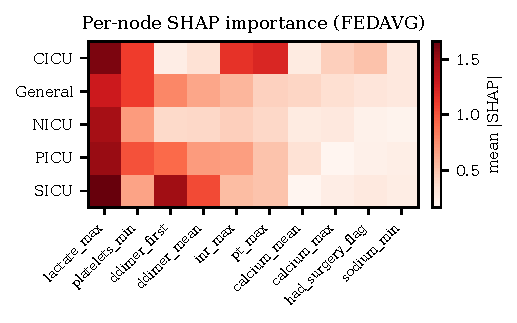
\includegraphics[width=0.88\textwidth]{figures/fig_node_shap_heatmap.pdf}
\caption{Per-node mean $|$SHAP$|$ across the top federated clinical features.}
\label{fig:heatmap}
\end{figure}

\subsection{Node vs. Federated Agreement}
Table \ref{tab:node-agreement} and Fig. \ref{fig:agreement} present the concordance between each local node's feature attributions and the aggregated federated ranking.

\begin{table}[t]
\caption{Spearman rank correlation, node ranking vs.\ federated aggregate (FedAvg)}
\label{tab:node-agreement}
\centering
\begin{tabular}{lcc}
\hline
\textbf{Node} & \textbf{Spearman $\rho$} & \textbf{$p$-value} \\
\hline
CICU    & 0.9297 & $1.10\times10^{-98}$  \\
NICU    & 0.9498 & $1.77\times10^{-114}$ \\
PICU    & 0.9739 & $1.47\times10^{-145}$ \\
SICU    & 0.9661 & $4.16\times10^{-133}$ \\
General & 0.9704 & $1.48\times10^{-139}$ \\
\hline
\end{tabular}
\end{table}

\begin{figure}[t]
\centering
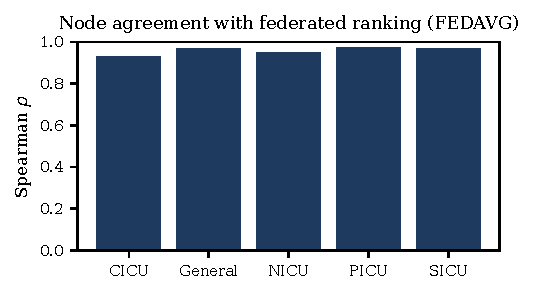
\includegraphics[width=0.88\textwidth]{figures/fig_node_agreement.pdf}
\caption{Spearman rank correlation of each node's local SHAP ranking against the federated aggregate.}
\label{fig:agreement}
\end{figure}

Every node correlates strongly with the federated aggregate, with Spearman $\rho$ ranging narrowly from 0.930 to 0.974. Notably, General ICU -- the dominant node at 49.4\% of all training data -- does \emph{not} show the highest agreement ($\rho = 0.970$, the second-highest of the five); that distinction belongs to PICU ($\rho = 0.974$). The \emph{lowest} agreement instead belongs to CICU, the smallest node at only 5.7\% of training data ($\rho = 0.930$), though even this minimum remains high in absolute terms. This is the opposite of the pattern that would indicate the federated aggregate is simply reproducing the dominant node's reasoning: if that were the case, General ICU's agreement would be near-perfect while the smaller nodes trailed well behind. Instead, all five nodes -- including both the largest and the smallest -- cluster within a 0.044 range of each other, suggesting the federated model has learned a reasoning pattern that generalizes across care-unit types rather than one dominated by whichever node contributed the most training data.

\subsection{Sensitivity Analysis: FedAvg vs.\ FedProx}
Figure \ref{fig:algo-compare} compares the federated feature ranking produced under each optimization algorithm. The two algorithms agree on 4 of their top 5 federated features -- \texttt{lactate\_max}, \texttt{platelets\_min}, \texttt{ddimer\_mean}, and \texttt{inr\_max} -- with an overall Spearman rank correlation across all 225 features of $\rho = 0.689$ ($p = 5.36\times10^{-33}$). While lower than the per-node agreement reported above, this still represents a strong positive correlation and confirms that the feature-importance pattern driving Sect. \ref{sec:results}'s findings is not an artifact of which federated optimizer was used to train the underlying model.

\begin{figure}[t]
\centering
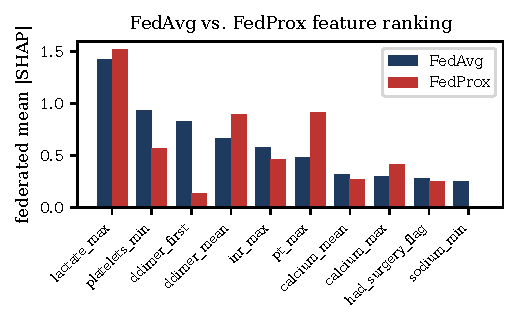
\includegraphics[width=0.88\textwidth]{figures/fig_fedavg_vs_fedprox.pdf}
\caption{Comparison of federated SHAP rankings under FedAvg versus FedProx.}
\label{fig:algo-compare}
\end{figure}

\section{Discussion}\label{sec:discussion}

The central empirical question this paper set out to answer was whether a federated model's explanation is trustworthy at every participating site, or only at the site that happened to contribute the most training data. The results in Sect. \ref{sec:results} answer this directly: node-level agreement with the federated aggregate is uniformly high (Spearman $\rho$ between 0.930 and 0.974) and does not track node size. If the federated SHAP aggregate were simply amplifying General ICU's reasoning, General ICU's own ranking should align with it almost perfectly while CICU, NICU, SICU, and PICU trailed visibly behind; instead, General ICU sits in the middle of the pack, and the smallest node, CICU, shows only a modestly lower -- still high -- correlation. This is a reassuring result for multi-site federated deployment: it suggests that aggregating SHAP values with the same sample-size weighting used for model updates does not inherit a bias toward the largest contributor's local feature distribution, at least under the care-unit-based non-IID partition evaluated here.

\texttt{lactate\_max} being the unanimous top feature across all five nodes reinforces this reading. Lactate is a direct marker of tissue hypoperfusion and a clinically well-established early indicator of septic shock; its consistent dominance across structurally different care units (a Cardiac ICU population and a Neonatal ICU population, for instance, have very different baseline physiology) is consistent with a model that has learned a genuine, generalizable physiological signal rather than a node-specific correlation. The FedAvg/FedProx agreement in Sect. \ref{sec:results} (4 of 5 top features shared, $\rho = 0.689$) provides a second, independent line of evidence for the same conclusion: even changing the federated optimization algorithm entirely leaves the core explanation largely intact.

These findings should be read as applying to the single sensitivity axis completed in this work -- the choice of federated algorithm -- and not yet to variation in cohort definition or node partitioning strategy, both of which remain open questions discussed below.

\subsection{Limitations and Future Work}\label{subsec:limitations}

The federated learning simulation partitions a single database by care-unit designation rather than drawing on genuinely separate institutional data sources; results here establish a lower bound on the practical cost of federation and of federated explainability, not a guarantee that a real multi-hospital deployment would behave identically. Of the three sensitivity axes designed for this work, only the algorithm-choice axis (FedAvg versus FedProx) was completed in time for this submission. The cohort-definition axis (re-running the full pipeline on the complete intermediate ICU cohort rather than the infection-restricted cohort used throughout) and the alternate-partition axis (grouping nodes by a criterion other than care-unit type, such as age band) were designed but not executed, and remain the most direct next steps for strengthening the robustness claims made in Sect. \ref{sec:discussion}.

\section{Conclusion}\label{sec:concl}

We introduced an interpretable federated SHAP architecture tailored for pediatric sepsis risk prediction, computing Shapley attributions locally at each of five simulated, non-IID ICU-type nodes and aggregating them with the same sample-size weighting used for federated model updates, without any node's raw patient data or per-patient attributions ever leaving that node. Across all five nodes, local SHAP rankings correlated strongly with the federated aggregate (Spearman $\rho$ between 0.930 and 0.974), with no evidence that the dominant node (49.4\% of training data) disproportionately shaped the aggregate explanation relative to the smallest node (5.7\%). \texttt{lactate\_max} emerged as the unanimous top feature at every node, and this finding was further confirmed as robust to the choice of federated optimization algorithm, with FedAvg and FedProx agreeing on 4 of their top 5 federated features. Together, these results suggest that per-node federated explainability is both practical to compute and trustworthy across heterogeneous clinical sites, at least along the one sensitivity axis evaluated to date. Extending this evaluation to cohort definition and alternate node partitioning, and validating the approach on genuinely separate institutional data rather than a simulated partition of a single database, are the natural next steps toward a deployable system.

\section*{Acknowledgment}
The investigators gratefully acknowledge the PhysioNet research consortium and the clinical curation teams responsible for hosting and maintaining the PIC database.

\bibliographystyle{splncs04}
\bibliography{references}

\end{document}
